\documentclass[a4paper,12pt]{article}

%%% Работа с русским языком % для pdfLatex
\usepackage{cmap}					% поиск в~PDF
\usepackage{mathtext} 				% русские буквы в~фомулах
\usepackage[T2A]{fontenc}			% кодировка
\usepackage[utf8]{inputenc}			% кодировка исходного текста
\usepackage[english,russian]{babel}	% локализация и переносы
\usepackage{indentfirst} 			% отступ 1 абзаца

%%% Работа с русским языком % для XeLatex
%\usepackage[english,russian]{babel}   %% загружает пакет многоязыковой вёрстки
%\usepackage{fontspec}      %% подготавливает загрузку шрифтов Open Type, True Type и др.
%\defaultfontfeatures{Ligatures={TeX},Renderer=Basic}  %% свойства шрифтов по умолчанию
%\setmainfont[Ligatures={TeX,Historic}]{Times New Roman} %% задаёт основной шрифт документа
%\setsansfont{Comic Sans MS}                    %% задаёт шрифт без засечек
%\setmonofont{Courier New}
%\usepackage{indentfirst}
%\frenchspacing

%%% Дополнительная работа с математикой
\usepackage{amsfonts,amssymb,amsthm,mathtools}
\usepackage{amsmath}
\usepackage{icomma} % "Умная" запятая: $0,2$~--- число, $0, 2$~--- перечисление
\usepackage{upgreek}

%%% Страница
\usepackage{extsizes} % Возможность сделать 14-й шрифт

%% Шрифты
\usepackage{euscript}	 % Шрифт Евклид
\usepackage{mathrsfs} % Красивый матшрифт

%% Свои команды
\DeclareMathOperator{\sgn}{\mathop{sgn}} % создание новой конанды \sgn (типо как \sin)
\usepackage{csquotes} % ещё одна штука для цитат
\newcommand{\pd}[2]{\ensuremath{\cfrac{\partial #1}{\partial #2}}} % частная производная
\newcommand{\abs}[1]{\ensuremath{\left|#1\right|}} % модуль
\renewcommand{\phi}{\ensuremath{\varphi}} % греческая фи
\newcommand{\pogk}[1]{\!\left(\cfrac{\sigma_{#1}}{#1}\right)^{\!\!\!2}\!}

% Ссылки
\usepackage{color} % подключить пакет color
% выбрать цвета
\definecolor{BlueGreen}{RGB}{49,152,255}
\definecolor{Violet}{RGB}{120,80,120}
% назначить цвета при подключении hyperref
\usepackage[unicode, colorlinks, urlcolor=blue, linkcolor=blue, pagecolor=blue, citecolor=blue]{hyperref} %синие ссылки
%\usepackage[unicode, colorlinks, urlcolor=black, linkcolor=black, pagecolor=black, citecolor=black]{hyperref} % для печати (отключить верхний!)
\mathtoolsset{showonlyrefs=true} % Показывать номера только у тех формул, на которые есть \eqref{} в~тексте.


%% Перенос знаков в~формулах (по Львовскому)
\newcommand*{\hm}[1]{#1\nobreak\discretionary{}
	{\hbox{$\mathsurround=0pt #1$}}{}}

%%% Работа с картинками
\usepackage{graphicx}  % Для вставки рисунков
\graphicspath{{images/}{images2/}}  % папки с картинками
\setlength\fboxsep{3pt} % Отступ рамки \fbox{} от рисунка
\setlength\fboxrule{1pt} % Толщина линий рамки \fbox{}
\usepackage{wrapfig} % Обтекание рисунков и таблиц текстом
\usepackage{multicol}

%%% Работа с таблицами
\usepackage{array,tabularx,tabulary,booktabs} % Дополнительная работа с таблицами
\usepackage{longtable}  % Длинные таблицы
\usepackage{multirow} % Слияние строк в~таблице
\usepackage{caption}
\captionsetup{labelsep=period, labelfont=bf}

%%% Оформление
\usepackage{indentfirst} % Красная строка
%\setlength{\parskip}{0.3cm} % отступы между абзацами

%%% Теоремы
\theoremstyle{plain} % Это стиль по умолчанию, его можно не переопределять.
\newtheorem{theorem}{Теорема}[section]
\newtheorem{proposition}[theorem]{Утверждение}

\theoremstyle{definition} % "Определение"
\newtheorem{definition}{Определение}[section]
\newtheorem{corollary}{Следствие}[theorem]
\newtheorem{problem}{Задача}[section]

\theoremstyle{remark} % "Примечание"
\newtheorem*{nonum}{Решение}
\newtheorem{zamech}{Замечание}[theorem]

%%% Правильные мат. символы для русского языка
\renewcommand{\epsilon}{\ensuremath{\varepsilon}}
\renewcommand{\phi}{\ensuremath{\varphi}}
\renewcommand{\kappa}{\ensuremath{\varkappa}}
\renewcommand{\le}{\ensuremath{\leqslant}}
\renewcommand{\leq}{\ensuremath{\leqslant}}
\renewcommand{\ge}{\ensuremath{\geqslant}}
\renewcommand{\geq}{\ensuremath{\geqslant}}
\renewcommand{\emptyset}{\varnothing}

%%% Название разделов
\usepackage{titlesec}


\usepackage{titlesec}
\titleformat{\section}{\normalfont\Large\bfseries}{}{0pt}{}


\title{Принцип работы лазера.}
\author{Гадецкий Дмитрий}
\date{Январь 2019}
\usepackage[left=1.35cm,right=1.35cm,top=1.4cm,bottom=2cm]{geometry}


\begin{document}
\maketitle
\thispagestyle{empty}
\newpage	 
Прежде чем переходить к рассмотрению принципов работы лазера, рассмотрим двухуровневую систему (рис \ref{fig:2sistem}). Пусть, для простоты, атом может принимать два состояния по энергии -- основное и возбужденное.
Рассмотрим систему из $N$ атомов при температуре $T$. 
Мы можем наблюдать три процесса: поглощение фотона, спонтанное излучение и вынужденное излучение. Разность энергий состояний атома такова, что:

\begin{equation}
h\nu = E_2-E_1
\label{eq_1}
\end{equation}

Мы сейчас не будем рассматривать кратные уровни энергий.
Пусть в основном состоянии находятся $n_1$ атомов, а в возбужденном $n_2$. В равновесии для системы будет справедливо распределение Больцмана.

\begin{equation}
n_i = n_{i0}\exp(-\frac{E_i}{kT})
\end{equation}

Вероятность самопроизвольного перехода частицы из верхнего состояния в нижнее пропорциональна времени. 
Частицы рассматриваемого ансамбля находятся в поле их собственного излучения, плотность энергии которого в единичном спектральном интервале составляет $\rho_{\nu}$. Это поле индуцирует переходы из верхнего состояния в нижнее и обратно.
Вероятность индуцированных переходов в единицу времени пропорциональна спектральной плотности энергии этого поля. Сказанное можно математически выразить следующим образом:

\begin{equation}
dw_{sp} = A_{21}dt
\end{equation}
\begin{equation}
dw_{12} = B_{12}\rho_{\nu}dt
\end{equation}
\begin{equation}
dw_{21} = B_{21}\rho_{\nu}dt
\end{equation}

Где $B_{12}$ = $B_{21}$ -- коэффициенты Энштейна.

\begin{figure}[h]
	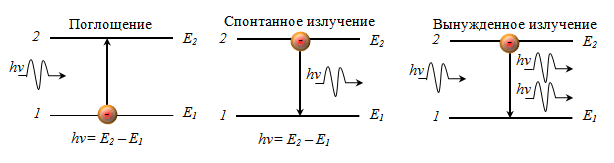
\includegraphics[width=\linewidth]{pict1.png}
	\caption{Двухуровневая система.}
	\label{fig:2sistem}
\end{figure}

Стоит пояснить, откуда берется равенство для коэффициентов Энштейна.
Если посмотреть на устройство лазера, в первом приближении, мы увидим, что это замкнутая полость с небольшим отверстием. В состоянии динамического равновесия это хорошая модель Абсолютно черного тела. Поместим и нашу двухуровневую систему в такие условия.
Излучение в нашей полости характеризуется спектральной плотностью $\rho(\omega,T)$, получаемой из формулы Планка:

\begin{equation}
\rho(\omega,T) = \frac{\hbar\omega^3}{\pi^2c^3}\cdot\frac{1}{\exp(\hbar\omega/kT)-1}
\end{equation}

Теперь запишем условия термодинамического равновесия нашей системы:
\begin{equation}
B_{12}\cdot\rho(\omega,T)n_1 = (A_{21}+B_{21}\cdot\rho(\omega,T))n_2
\end{equation}
%Figure \ref{fig:2sistem} shows a boat.
\newpage

Перепишем последнее условие с учетом распределения Больцмана:
\begin{equation}
B_{12}\cdot\rho(\omega,T)\cdot\exp(-E_1/kT) = (A_{21}+B_{21}\cdot\rho(\omega,T))\cdot\exp(-E_2/kT)
\end{equation}
Выражая отсюда $\rho(\omega,T)$ получаем:
\begin{equation}
\rho(\omega,T) = \frac{A_{21}}{B_{12}\exp(\hbar\omega/kT)-B_{21}}
\end{equation}

Так как при $T\longrightarrow \infty$ спектральная плотность излучения должна неограниченно возрастать, нам следует положить знаменатель равным нулю, откуда мгновенно получается равенство коэффициентов Энштейна.

Из уравнения термодинамического равновесия мы видим, что в такой системе $n_1$ всегда больше чем $n_2$. Идея же лазерного излучения потребует от нас инверсной заселенности энергетических уровней, и потому, не будет реализуема в такой системе. Сейчас мы переходим к рассмотрению подводящих к этому соображений.


Спонтанное излучение некогерентно. В этом случае атомы источника излучают независимо друг от друга. Лазер же работает на принципе индуцированного излучения. При переходе атома с энергетического уровня $E_2$ на $E_1$ под "действием" фотона, излученный фотон ему полностью идентичен. Теперь становится понятным, зачем нам нужна инверсная заселенность. Рассмотрим предельный случай, когда $n_2 \gg n_1$. Пусть произошел некоторый спонтанный переход. Фотон, излученный при этом стимулирует излучение соседних атомов когерентным образом и получается, своего рода, лавинообразный эффект.
На торцах трубки лазеров устанавливаются зеркала с очень хорошей отражающей способностью, что значительно усиливает данный эффект.

Собственно вопрос в том, как именно создать в нашей системе инверсную заселенность.
Существует достаточно много таких систем, отдавая дань истории мы рассмотрим принцип работы рубинового лазера.

Рубин -- это кристалл корунда $Al_2O_3$, в котором небольшая часть атомов алюминия замещена атомами хрома $Cr^{3+}$, порядка $0.05 \%$ по массе. Корунд, который в данном случае играет роль твердого “растворителя” для ионов хрома, выбран не случайно. Он прозрачен для световых волн, использующихся как для возбуждения ионов хрома, так и для самого лазерного излучения. Электронная конфигурация иона $Cr^{3+}$
имеет следующую структуру: $1s^22s^22p^63s^23p^63d^3$. В свободно ионе формируется 
шесть дублетных  ${}^2P$,${}^2D$,${}^2F$,${}^2G$,${}^2H$ и два квартетных ${}^4P$,${}^4F$ по спину терма. Нижним термом и ближайшим к нему являются соответственно ${}^4F$ $S=3/2, L=3$ и ${}^2G$ $S=1/2, L=4$. Количество подуровней с одинаковой энергией, определяется формулой $g=(2S+1)(2L+1)$ и составляет для этих термов 28 и 18.

В кристаллической решетке рубина ионы хрома имеют отличную структуру уровней энергии, от той, которой обладают свободные ионы. Каждый ион хрома окружен шестью ионами $O^{2-}$, находящимися в вершинах октаэдра, и создающими в месте расположения иона хрома сильное электрическое поле  (рис \ref{fig:2sistem1}). 

\begin{figure}[h!]
	\centering
	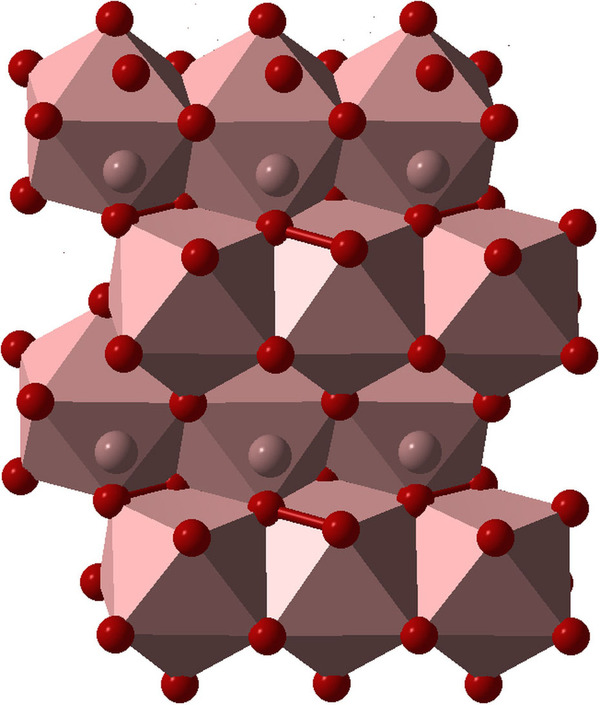
\includegraphics[scale=0.2]{pict2.png}
	\caption{Кристаллическая решетка рубина.}
	\label{fig:2sistem1}
\end{figure}
\newpage

В сильном поле октаэдрической симметрии ${}^4F$ терм расщепляется на три подуровня --
один орбитальный синглет ${}^4A_2$ и два орбитальных триплета ${}^4T_1$ и ${}^4T_2$.
Уровни ${}^4T_1$ и ${}^4T_2$  расщепляются на ряд перекрывающихся дублетов, образуя широкие полосы энергетических состояний. В свою очередь терм ${}^2G$ в кристаллическом поле расщепляется на 4 группы уровней. Самый нижний уровень, обозначаемый как ${}^2E$, вовлечен в процесс лазерной генерации в роли верхнего уровня лазерного перехода. Он состоит из двух подуровней, обозначаемых $2A$ и $E$, которые разнесены по энергии на 29 $cm^{-1}$ (рис \ref{fig:2sistem2}).

\begin{figure}[h!]
	\centering
	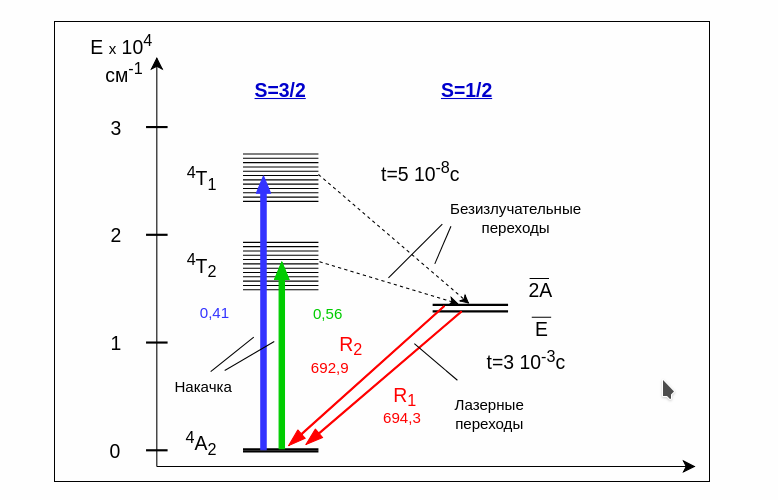
\includegraphics[scale=0.7]{pict3.png}
	\caption{Расщепленные уровни энергий.}
	\label{fig:2sistem2}
\end{figure}

Рубиновый лазер работает по трехуровневой схеме. При комнатной температуре населен только нижний уровень ${}^4A_2$.  Накачка в первых и некоторых последующих моделях лазера осуществлялась широкополосным излучением ксеноновой лампы-вспышки с этого уровня на группы ${}^4T_1$ и ${}^4T_2$. Это сильные разрешенные переходы, так как состояния имеют разные электронные конфигурации и одинаковый спин. Поглощение происходит в зеленой и фиолетовой областях видимого света с центрами 0.56 и 0.41 мкм. Ширина полос поглощения порядка 100 нм. Эти полосы хорошо наблюдаются в обычном спектре поглощения рубина.

 С возбужденных состояний ионы хрома стремятся различными способами перейти на нижележащие уровни. Безызлучательные переходы между состояниями ${}^4T_1$, ${}^4T_2$ и состоянием ${}^2E$ имеют намного большую вероятность, чем прямые переходы в основное состояние. Время жизни верхних уровней мало и порядка $5\cdot10^-8$ секунды. Переход ${}^2E \longrightarrow {}^4A_2$запрещён в дипольном приближении, так как орбитали этих уровней имеют одну и ту же конфигурацию, и кроме того он запрещён по спину. Поэтому уровень ${}^2E$ является метастабильным и время жизни такого состояния для атома на несколько порядков дольше. Это позволяет запасать в таком состоянии большую энергию.
 
  Каждый из двух подуровней $2A$ и $E$   мог бы быть верхним уровнем соответствующего лазерного перехода. Однако, в силу быстрой взаимной релаксации, со временем порядка $10^{-8}$ секунды, на этой паре уровней устанавливается определенное термическое равновесие, при котором населённость нижнего уровня 
 значительно выше населённости верхнего.
 
\begin{figure}[h!]
	\centering
	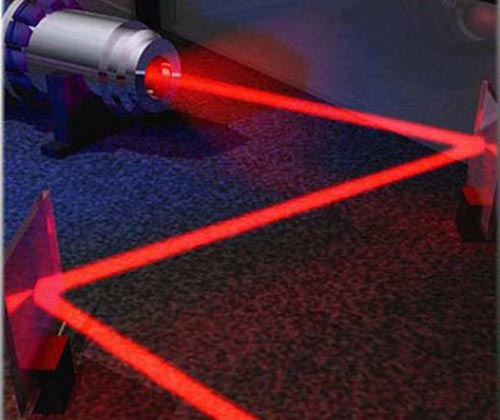
\includegraphics[scale=2]{pict4.png}
	\caption{Рубиновый лазер в действии.}
	\label{fig:2sistem3}
\end{figure}

Таким образом в рубиновом лазере создается инверсная заселенность, которая позволяет получать за счет многократного отражения от зеркал пучек излучения в очень узком спектре.
\end{document}
